\documentclass[12pt,aspectratio=169]{beamer}


\usepackage{algorithm,algorithmic}

\usepackage[utf8]{inputenc}
\usepackage{booktabs}
\usepackage[opacity=0.1]{pdfcomment} % set to 0 to make annotation icons invisible
\usepackage{pdfpc}
\usepackage{arev}
\usepackage{multicol}

\usepackage{xcolor, color, colortbl}
\definecolor{dkgreen}{rgb}{0,0.5,0}
\definecolor{dkred}{rgb}{0.8,0,0}
\definecolor{dkblue}{rgb}{0,0,0.5}
\definecolor{gray}{rgb}{0.5,0.5,0.5}
\definecolor{mauve}{rgb}{0.58,0,0.82}
\definecolor{hilight}{RGB}{122,86,0}

\definecolor{LRed}{rgb}{1,.8,.8}
\definecolor{MRed}{rgb}{1,.6,.6}
\definecolor{HRed}{rgb}{1,.2,.2}

\usepackage{tikz}
\usetikzlibrary{arrows.meta,
                calc, chains,
                quotes,
                positioning,
                shapes.geometric}


\def\scalefact{0.85}
\newcommand{\cev}[1]{\reflectbox{\ensuremath{\vec{\reflectbox{\ensuremath{#1}}}}}}
\newcommand{\evalat}[2]{\left.#1\right\vert_{#2}}

\newcommand{\znode}[5][black]{\path (#3,#4) node(#2) [circle,draw,color=#1] {#5};}
\newcommand{\zunedge}[6][black]{%
\begin{scope}
	\path (#2,#3) node(this) [inner sep=0pt,triangle,draw,color=#1] {#4};
	\draw[->,color=#1] (#5) -- (this.west);
	\draw[->,color=#1] (this.east) -- (#6);
\end{scope}}
\newcommand{\zbiedge}[7][black]{%
\begin{scope}
	\path (#2,#3) node(this) [inner sep=0pt,triangle,draw,color=#1] {#4};
	\draw[->,color=#1] (#5) -- (this);
	\draw[->,color=#1] (#6) -- (this);
	\draw[->,color=#1] (this.east) -- (#7);
\end{scope}}
\newcommand{\zedge}[5][black]{\path (#3,#4) node(#2) [inner sep=0pt,triangle,draw,color=#1] {#5};}

\definecolor{blue(pigment)}{rgb}{0.2, 0.2, 0.6}
\definecolor{burgundy}{rgb}{0.5, 0.0, 0.13}


\usepackage{listings}
%% \usetheme{Goettingen}
\usefonttheme{serif}
\usepackage{times}
\setbeamertemplate{navigation symbols}{}

\title{Deep Learning}
\subtitle{Lecture 8: Test Sets, Validation Sets, and Overfitting}
 
 
%\author[Mehrdad Maleki] % (optional, for multiple authors)
%{Mehrdad Maleki, Barak A. Pearlmutter\footnote{ Institute & Department of Computer Science
%Maynooth University, Co. Kildare, Ireland}, Jeffrey Mark Siskind}
 
%\institute[NUIM] % (optional)
%{
%  Department of Computer Science \\
%  National University of Ireland Maynooth
 
%}

\author[]{\textbf{Dr. Mehrdad Maleki}}
%\institute[]{\textsuperscript{1}Department of Computer Science\\ National University of Ireland\\ Maynooth}
 
\date{}
 
%\logo{\includegraphics[height=1.5cm]{lion-logo.png}}

\renewcommand{\Re}{\mathbb{R}}
 
\begin{document}
 
\frame{\titlepage}

\begin{frame}
\frametitle{}
Consider the following data $(x,y)$. 
\begin{center}
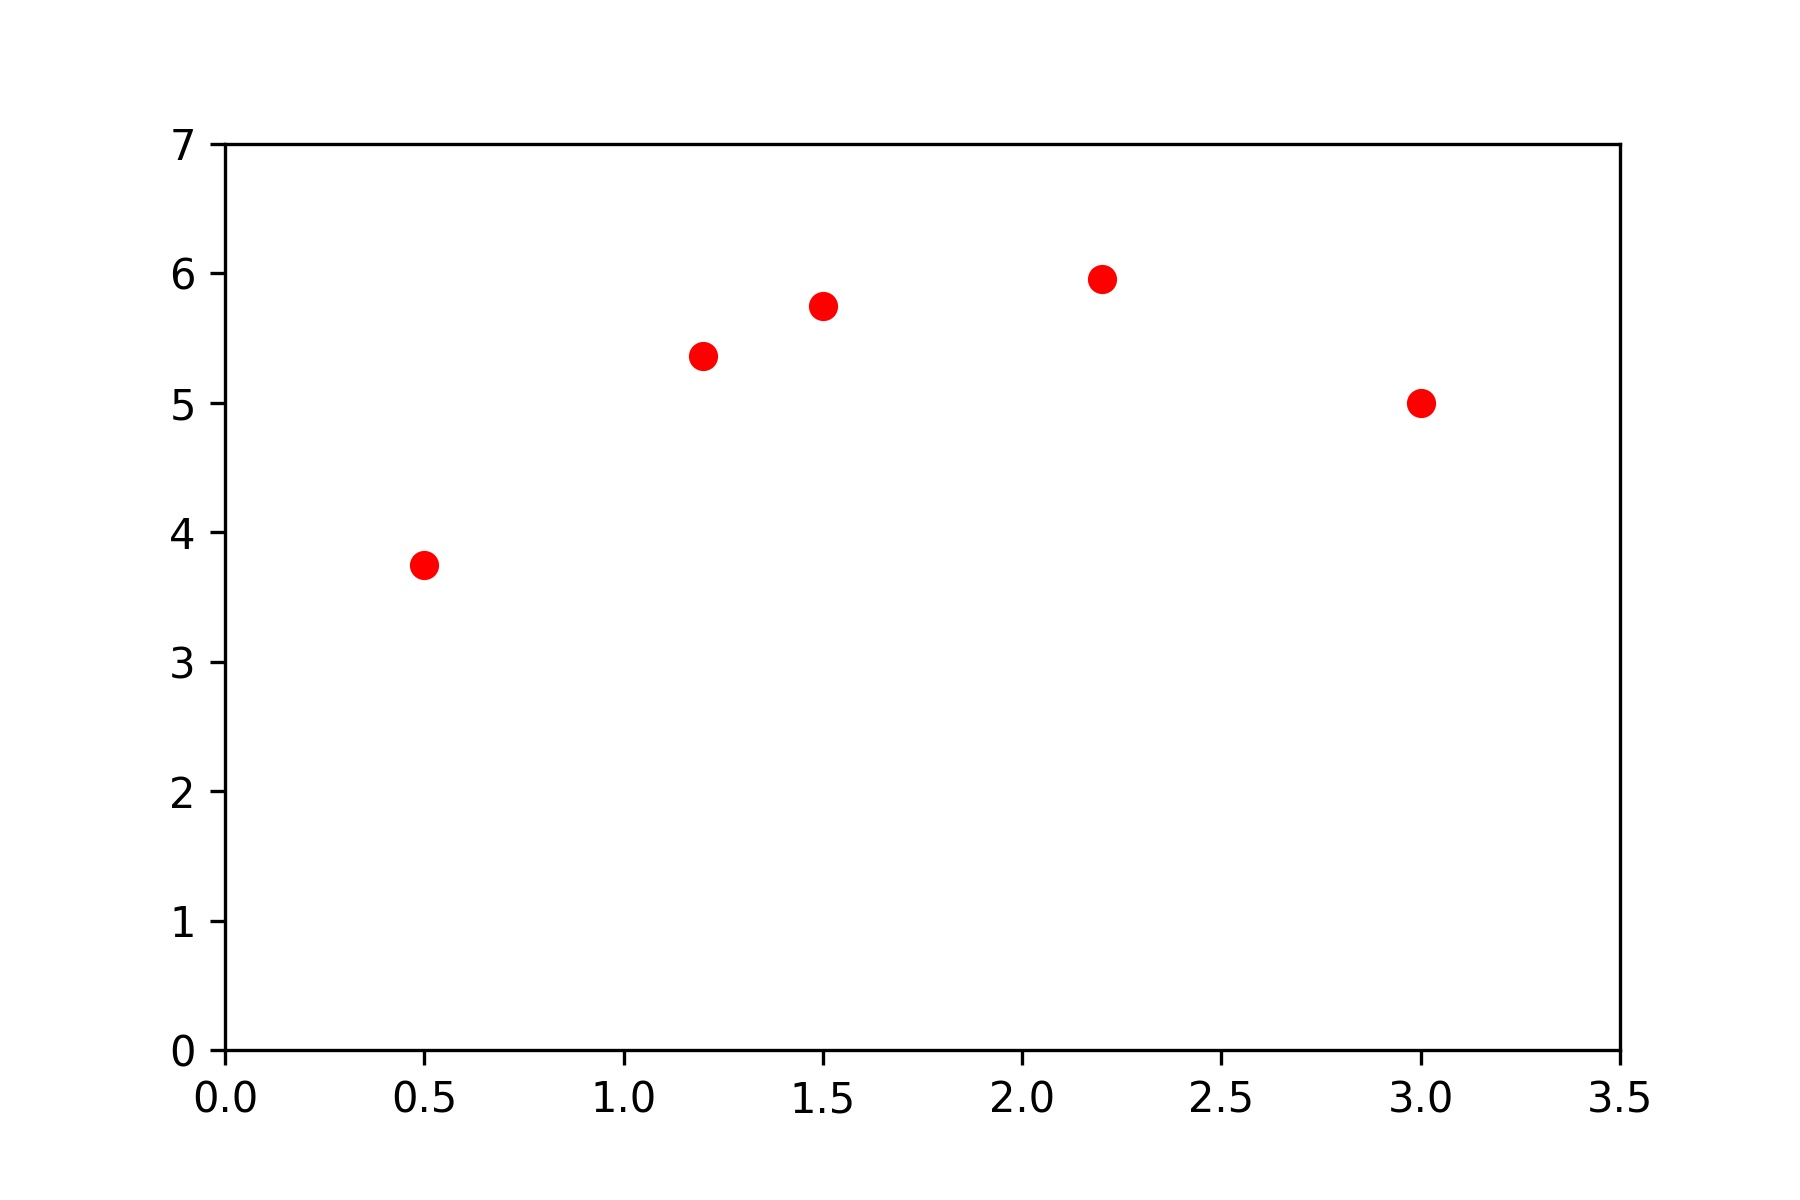
\includegraphics[scale=0.7]{Quadratic}
\end{center}
\end{frame}

\begin{frame}
We can model this data by the following estimators,
\begin{enumerate}
\item Linear estimator, i.e., $\hat{y}=w_0+w_1x$\pause
\bigskip
\item Quadratic estimator, i.e., $\hat{y}=w_0+w_1x+w_2x^2$\pause
\bigskip
\item Higher order estimator, i.e., $\hat{y}=\sum_{i=0}^{20}w_ix^i$
\end{enumerate}
\end{frame}

\begin{frame}
If we use linear estimator we have,
\begin{center}
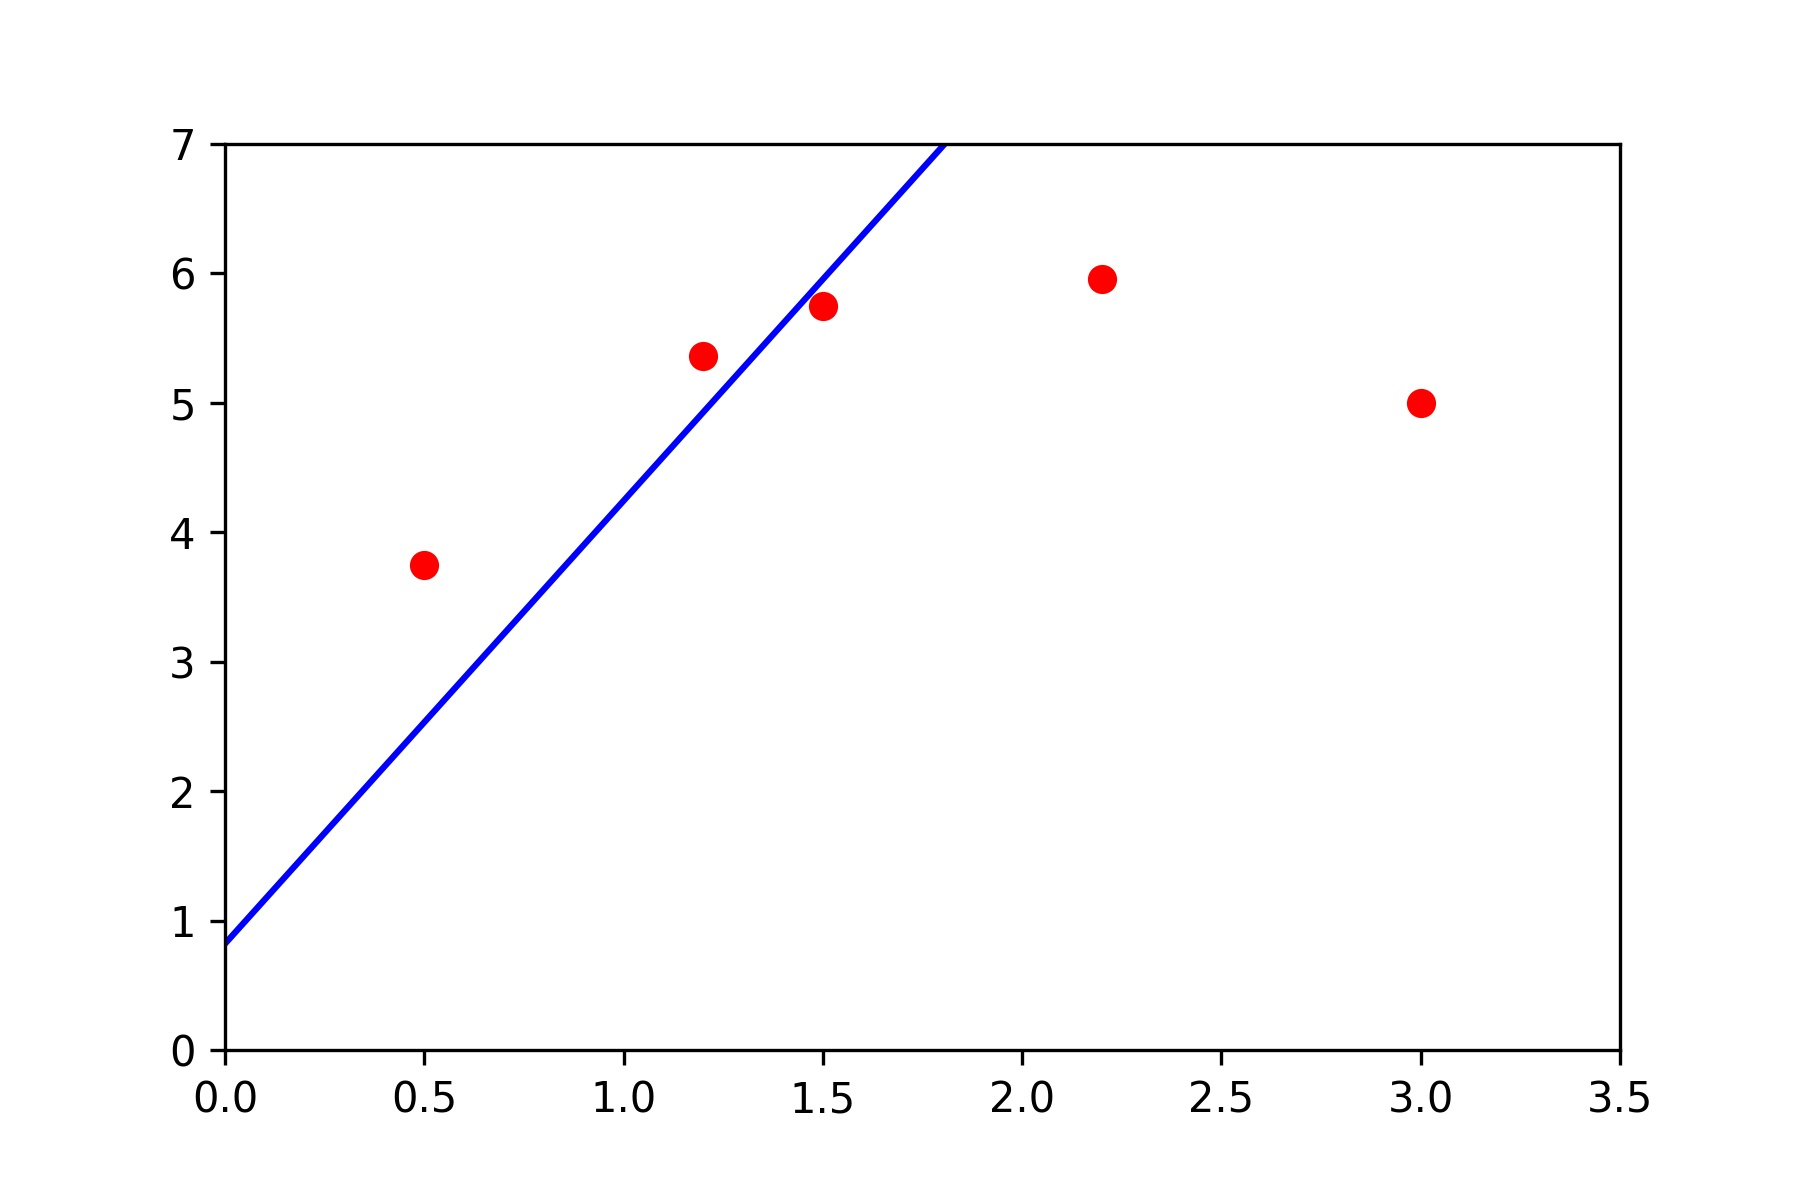
\includegraphics[scale=0.7]{Linear}
\end{center}
\end{frame}


\begin{frame}
If we use Quadratic estimator we have,
\begin{center}
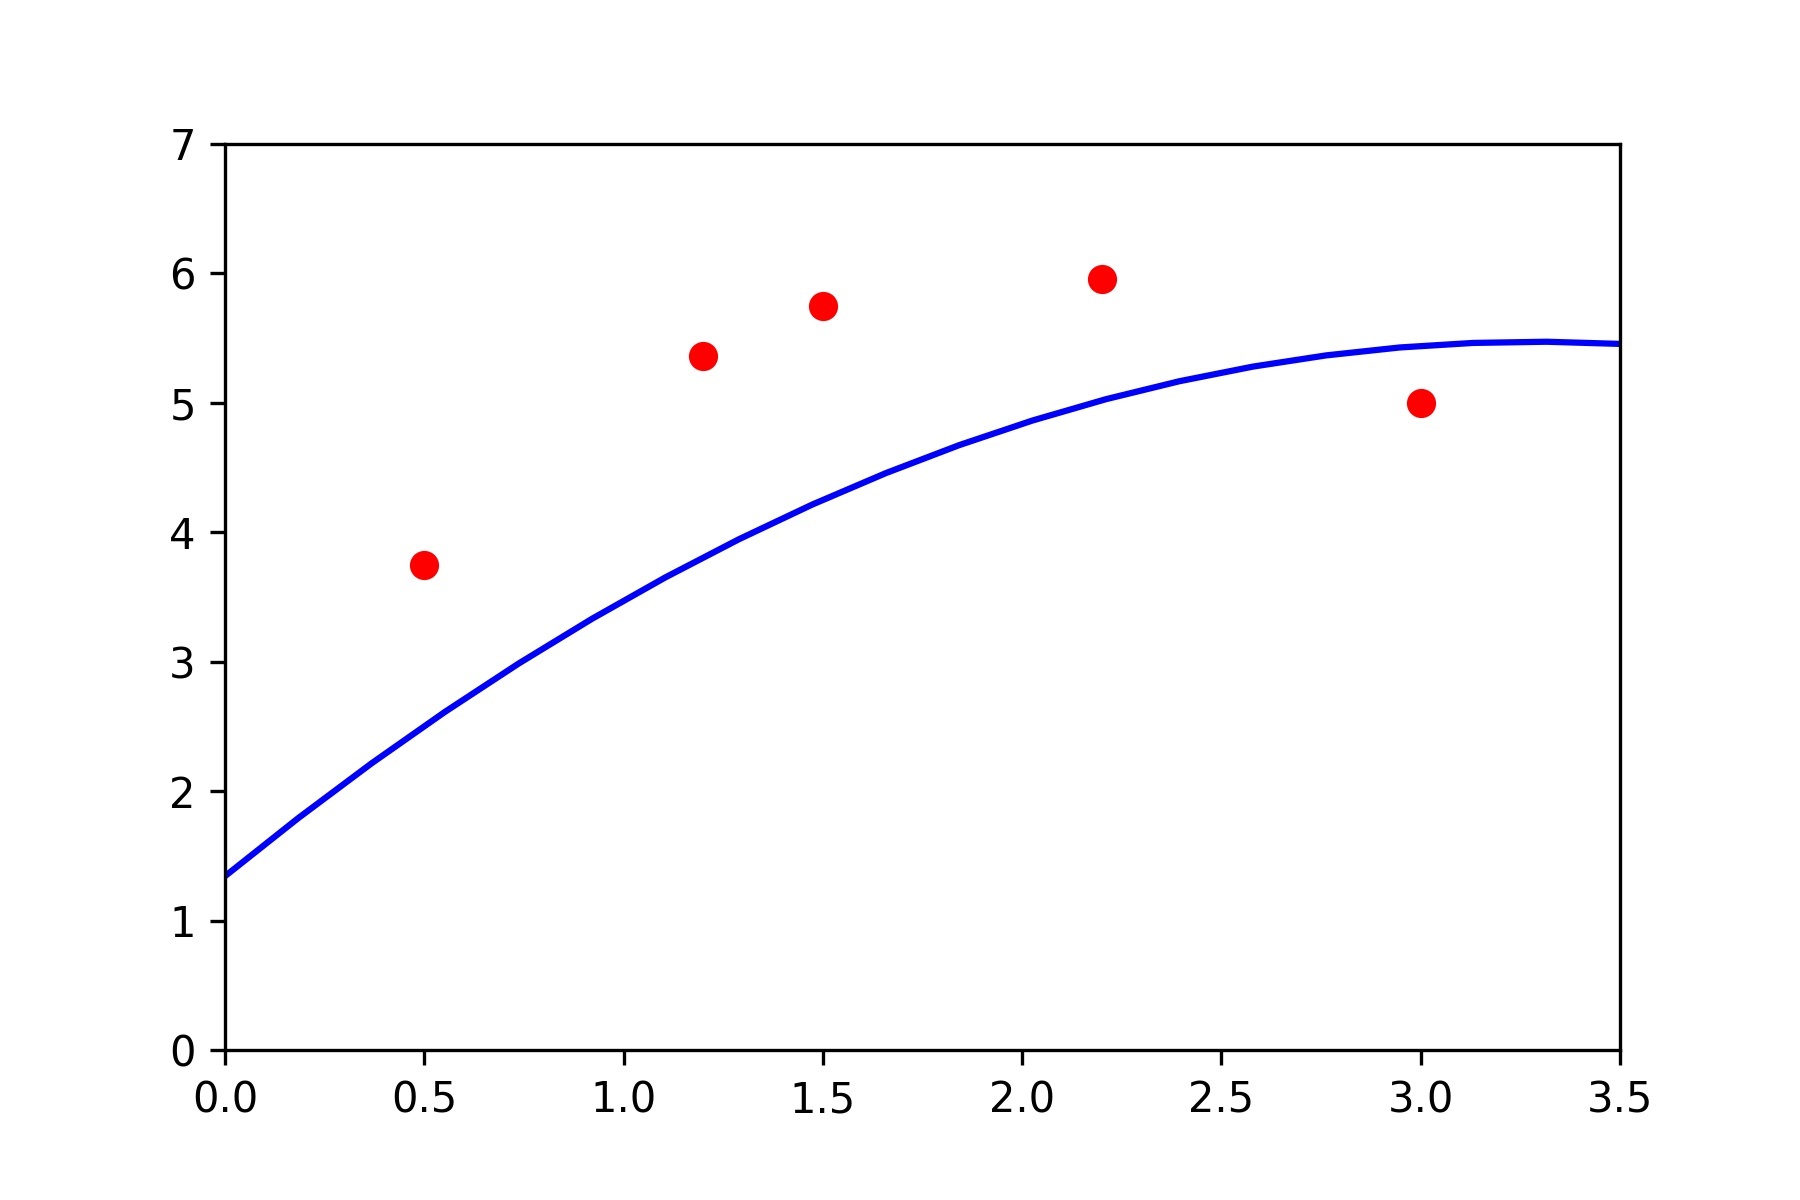
\includegraphics[scale=0.7]{Quadratic3}
\end{center}
\end{frame}


\begin{frame}
If we use polynomail of degree 5 estimator we have,
\begin{center}
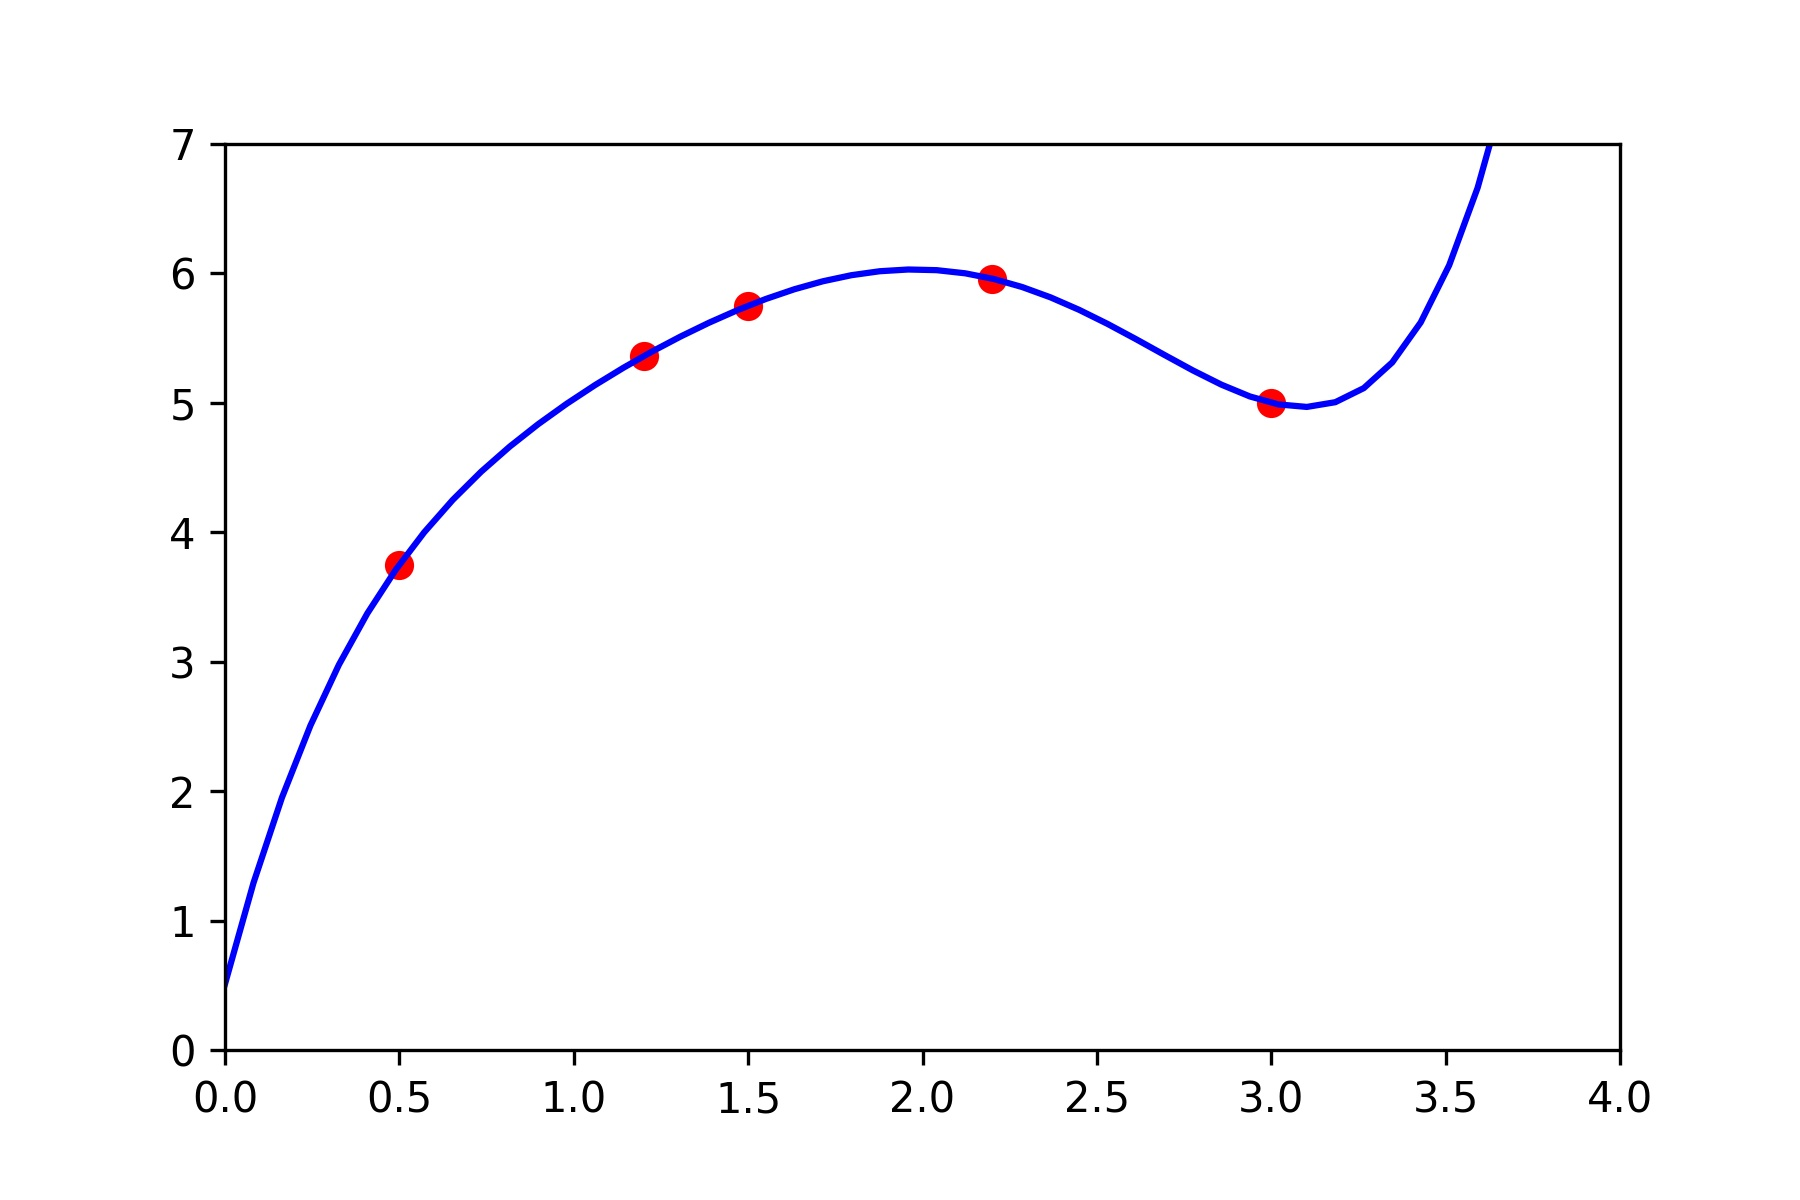
\includegraphics[scale=0.7]{Quadratic4}
\end{center}
\end{frame}

\begin{frame}
\begin{enumerate}
\item 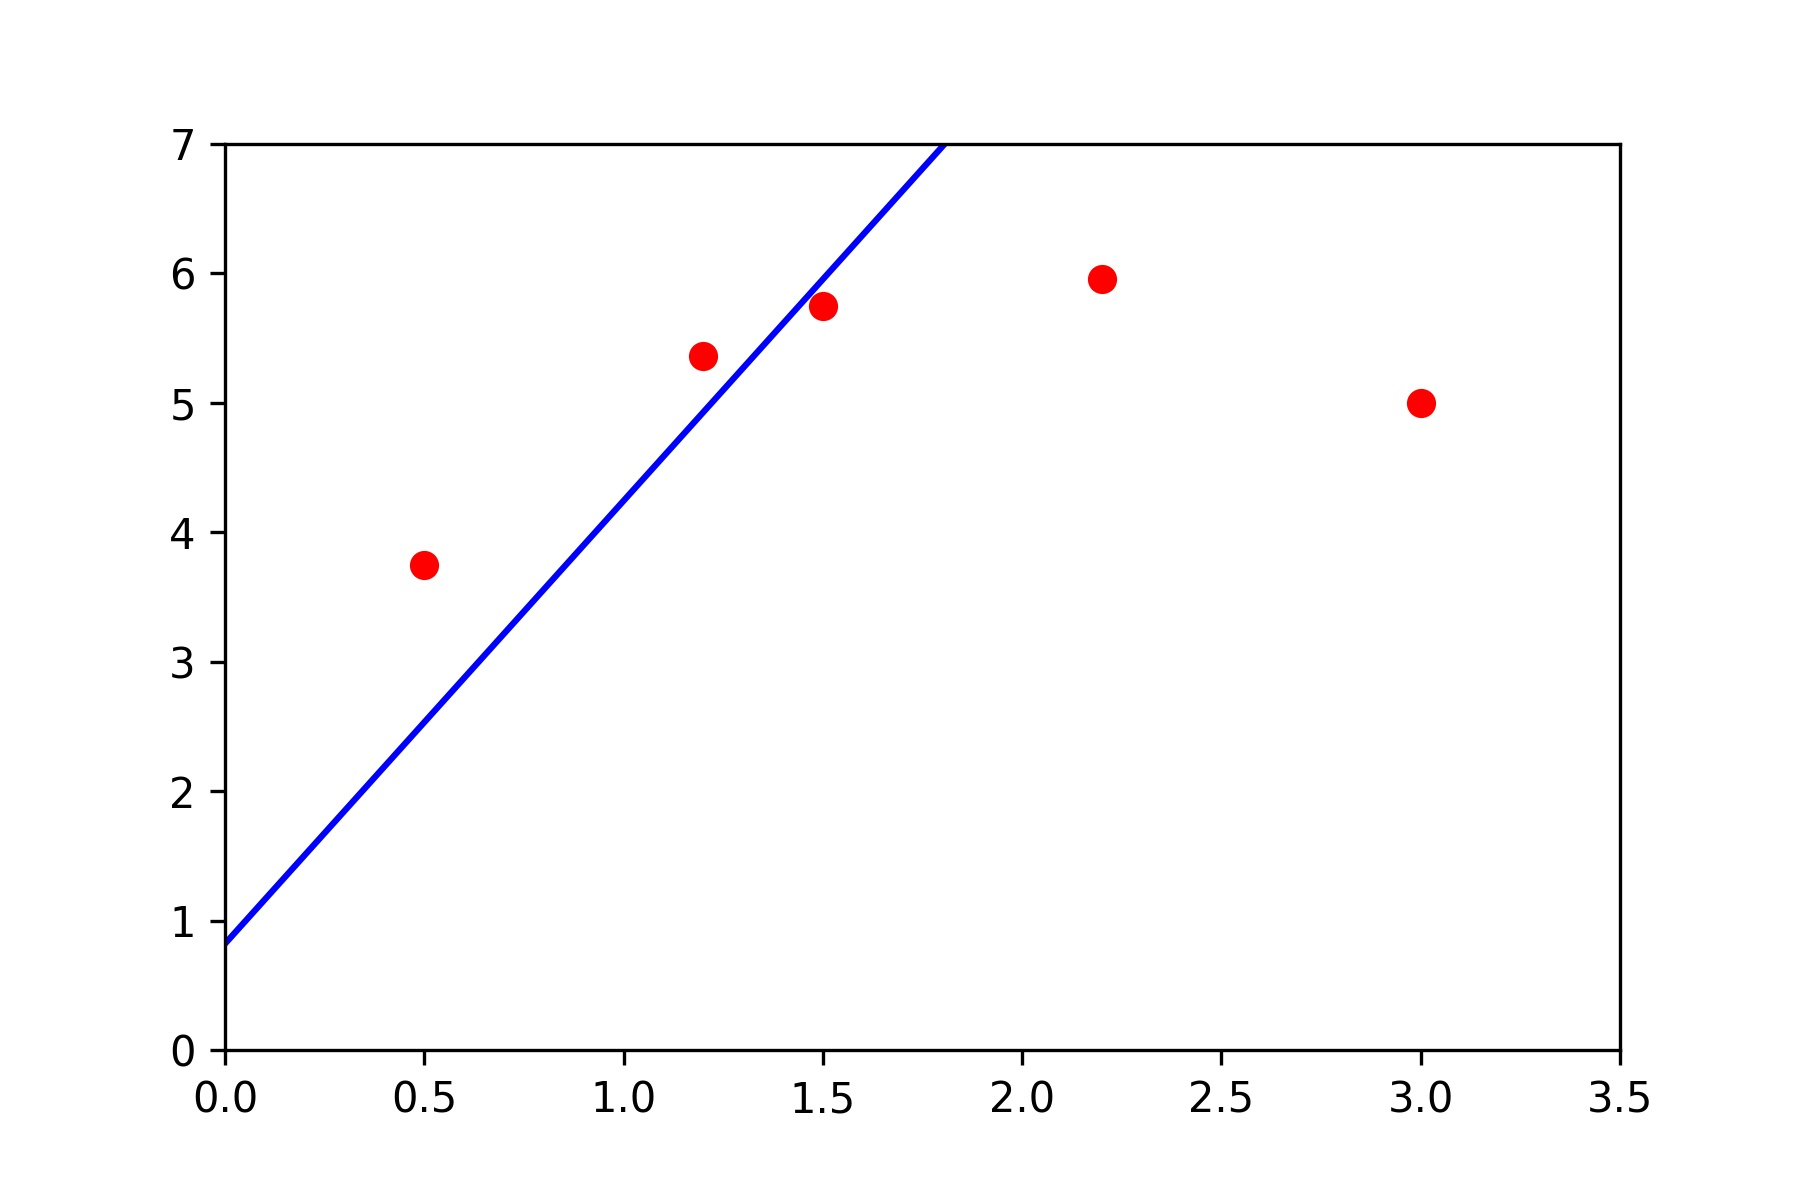
\includegraphics[scale=0.2]{Linear} \textbf{Underfitting}\pause
\item 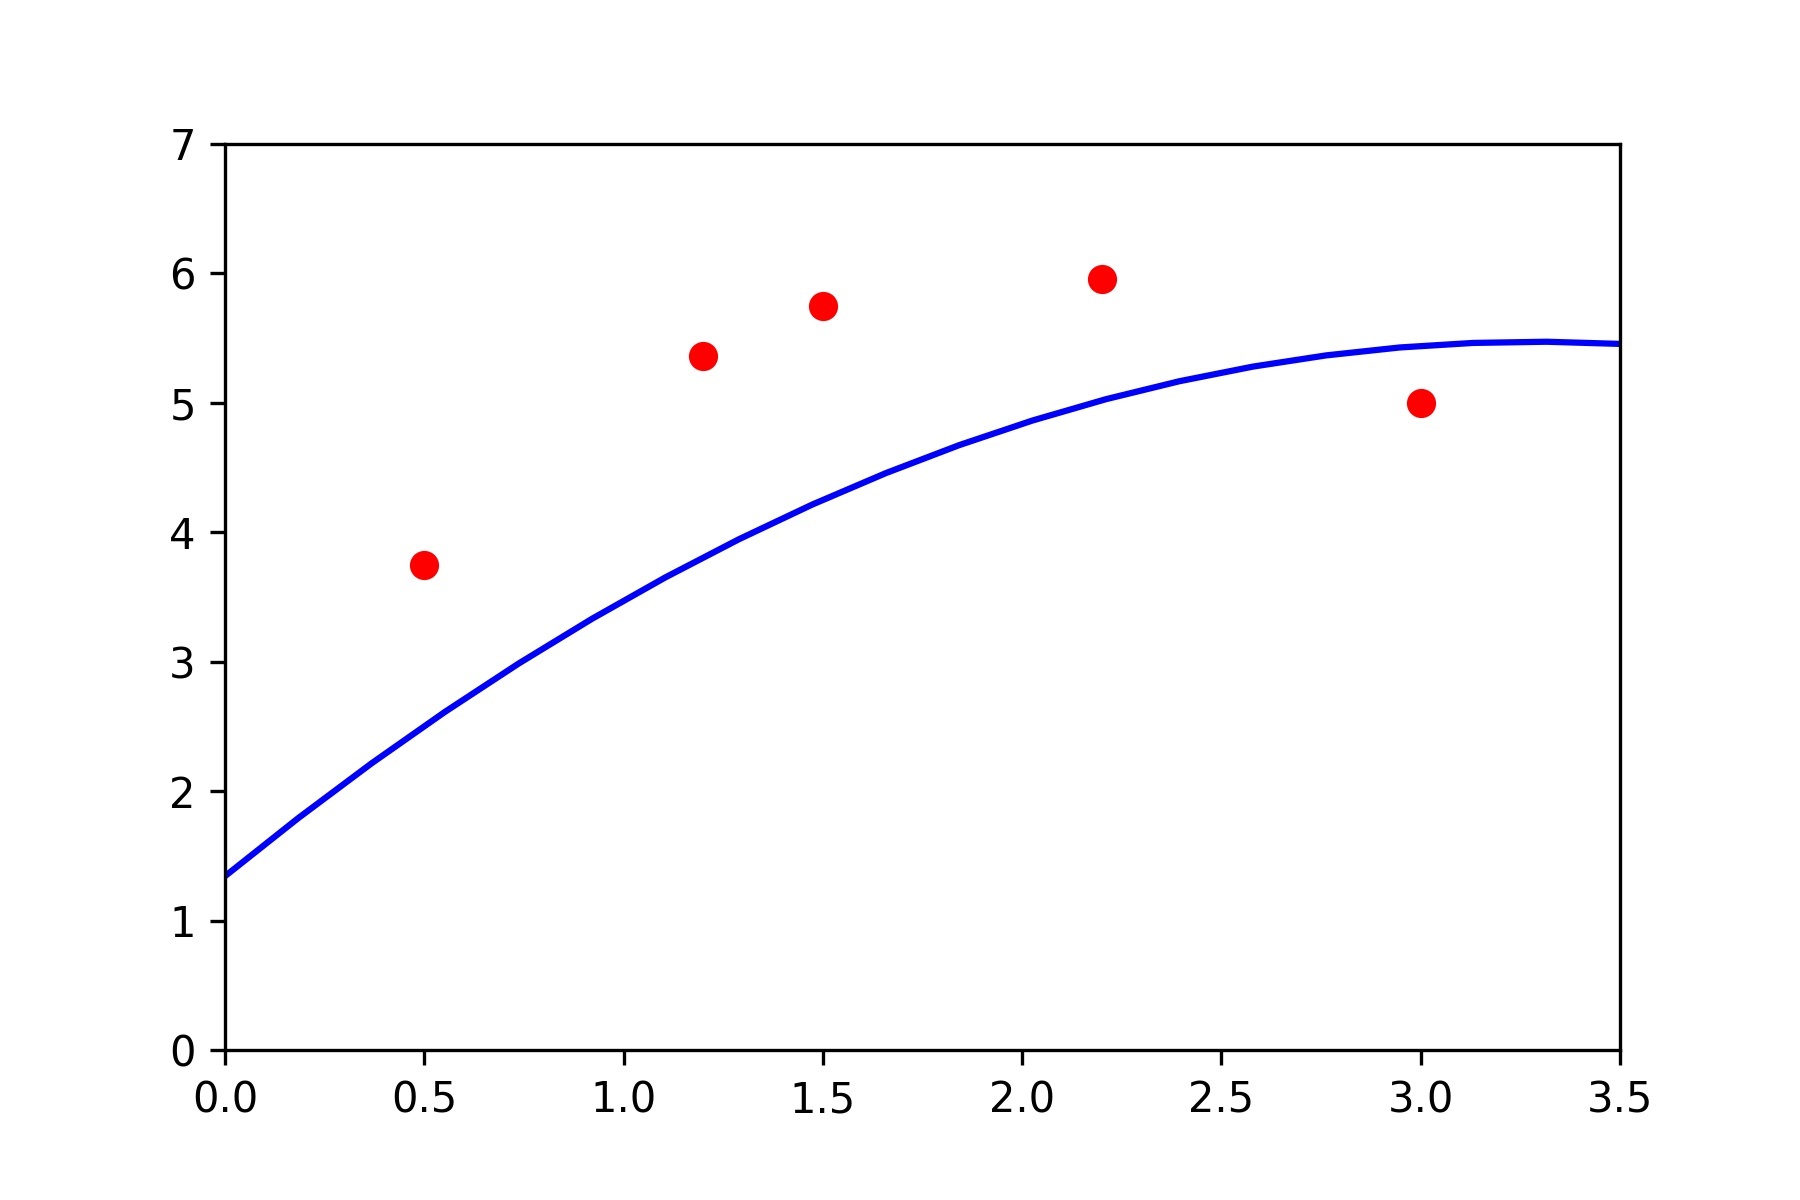
\includegraphics[scale=0.2]{Quadratic3} \textbf{Appropriate Capacity}\pause
\item 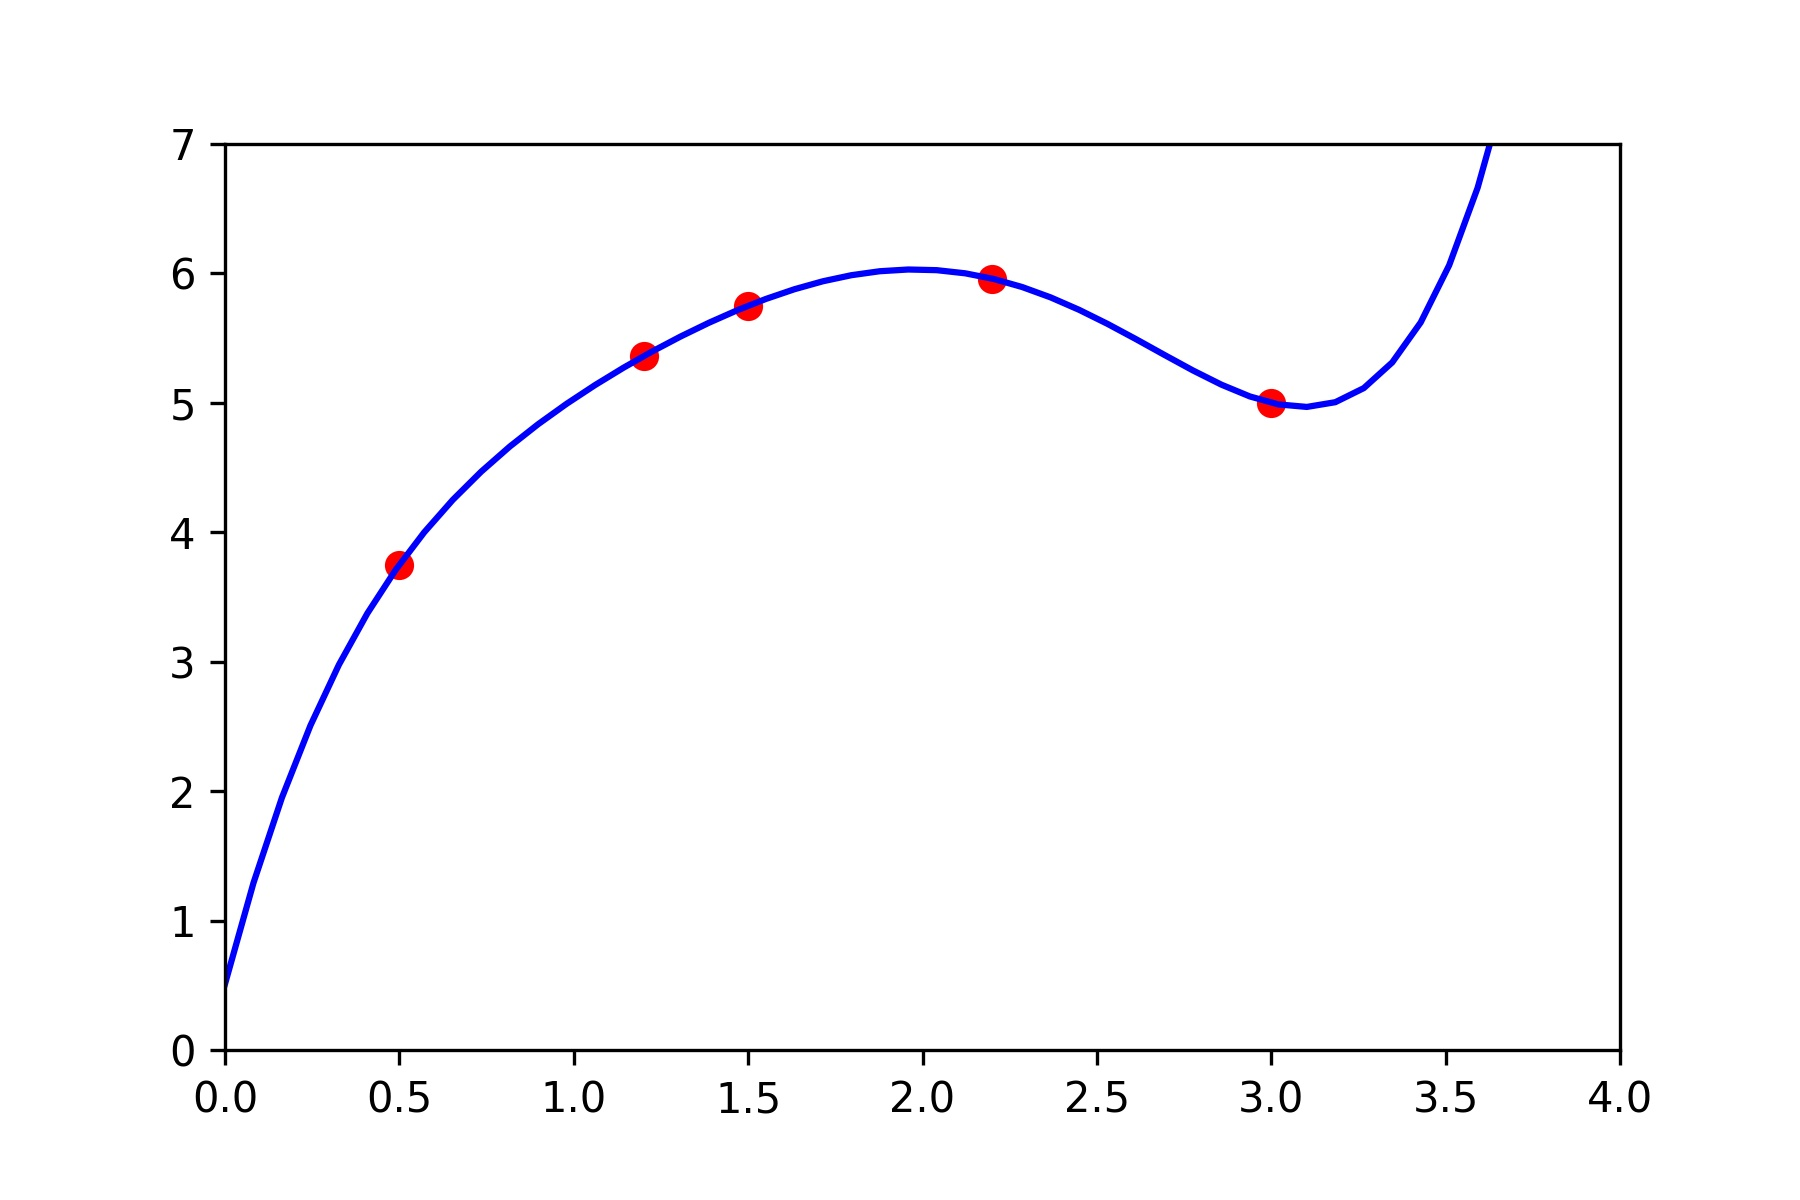
\includegraphics[scale=0.2]{Quadratic4} \textbf{Overfitting}
\end{enumerate}
\end{frame}

\begin{frame}
\frametitle{Generalization error}
The \textbf{generalization error (test error)} is defined as the expected value of the error on a new input. Here the expectation is taken across different possible inputs.  
\end{frame}

\begin{frame}
The factors determining how well a machine learning algorithm will perform are its ability to:
\begin{enumerate}
\item Make the training error small.
\bigskip
\item Make the gap between training and test error small.
\end{enumerate}
Thus
\begin{enumerate}
\item \textbf{Underfitting:}model is not able to obtain a sufficiently low error value on the trainig set.
\bigskip
\item \textbf{Overfitting:}the gap between the training error and test error (\textbf{generalization gap}) is too large.
\end{enumerate}
\end{frame}

\begin{frame}
\begin{center}
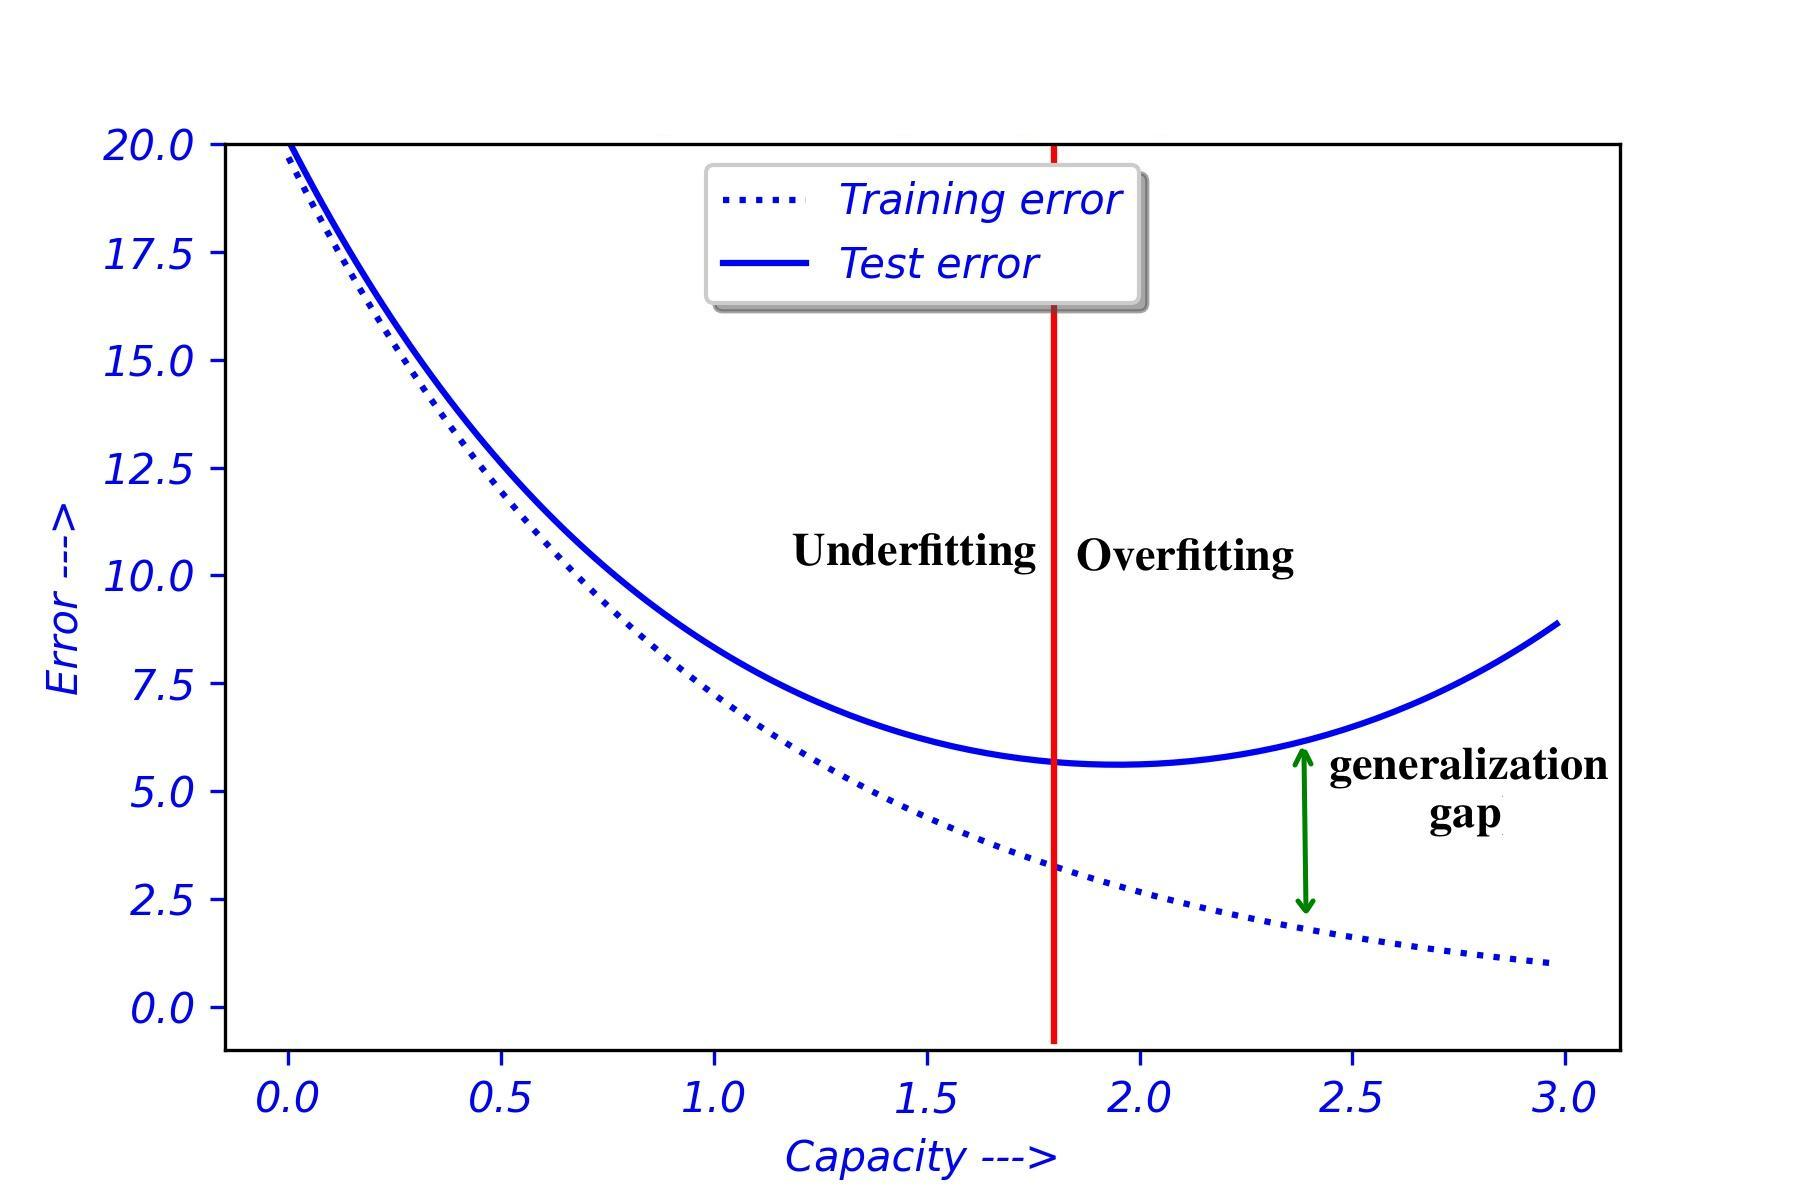
\includegraphics[scale=0.8]{Overfitting}
\end{center}
\end{frame}



\begin{frame}
\begin{center}
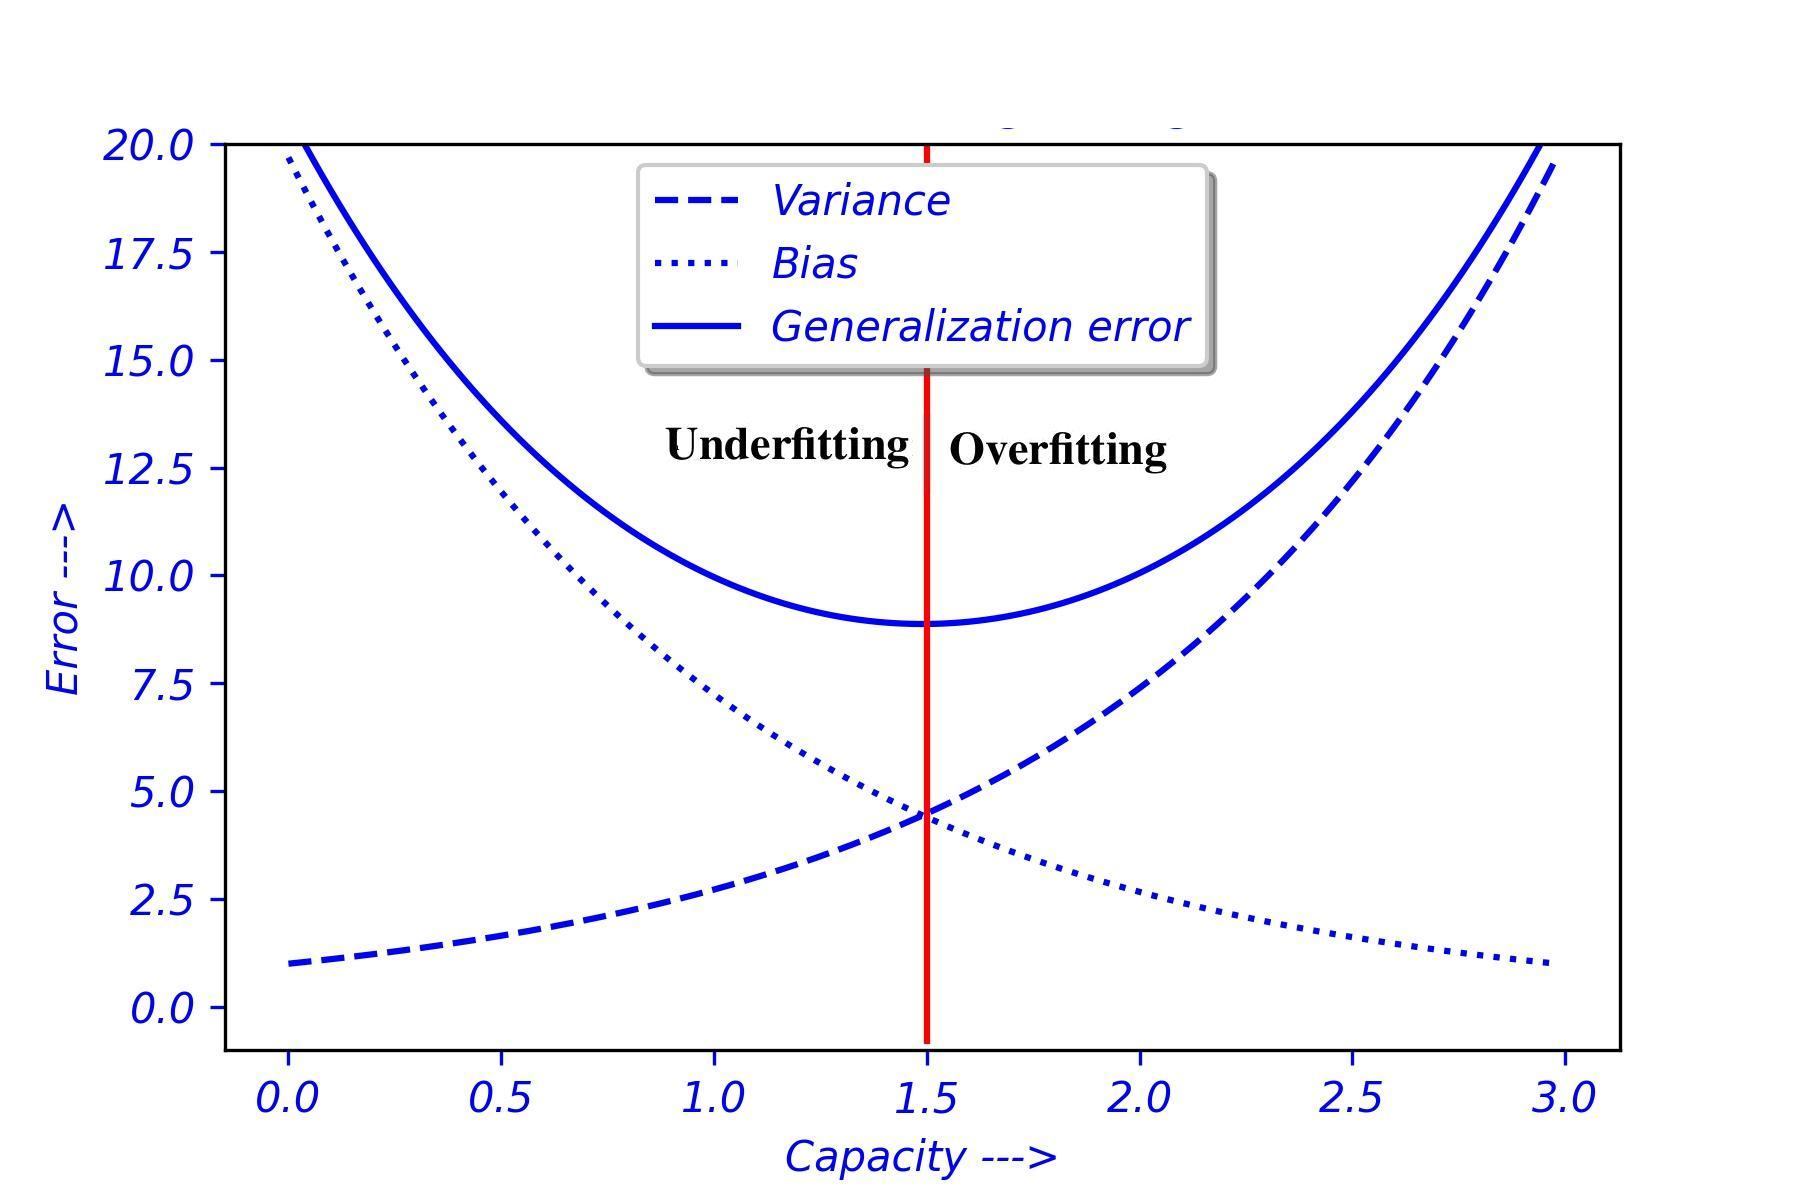
\includegraphics[scale=0.8]{Bias}
\end{center}
\end{frame}

\begin{frame}{}
  \centering \Huge
  \emph{Thank You}
\end{frame}

\end{document}

